\documentclass[10pt,a4paper,titlepage]{article}
\usepackage[utf8]{inputenc}

\usepackage{amsmath}
\usepackage{amsfonts}
\usepackage{amssymb}
\usepackage{graphicx}
\usepackage{float} % force figure to render inline location
\usepackage{enumitem} % apt install texlive-latex-extra 
\usepackage{anyfontsize} % custom fontsizes
\usepackage{titlesec} % custom section spacings
\usepackage{multirow} % merge table rows
\usepackage{vhistory} % revision table package
\usepackage{pdfpages}

\setlist[itemize]{noitemsep} % No spaces in itemize lists
\setlist[enumerate]{noitemsep} % No spaces in itemize lists
\setlist[description]{noitemsep} % No spaces in itemize lists
\titlespacing*{\subsubsection}{0pt}{8pt}{2pt}
\titlespacing*{\paragraph}{0pt}{3pt}{5pt}

\newcommand{\cpright}{\textsuperscript{\tiny\copyright}}

\setlength\parindent{0pt}

\begin{document}
	
	\begin{titlepage}
		
		\title{
			\fontsize{50}{12}\selectfont{\textsc{Lunar Rover}}\\
			\vspace{20pt}
			\fontsize{20}{12}\selectfont{\textsc{User Manual}}\\
			\vspace{10pt}
			\large{Software Engineering \& Project} \\
			\vspace{20pt}
			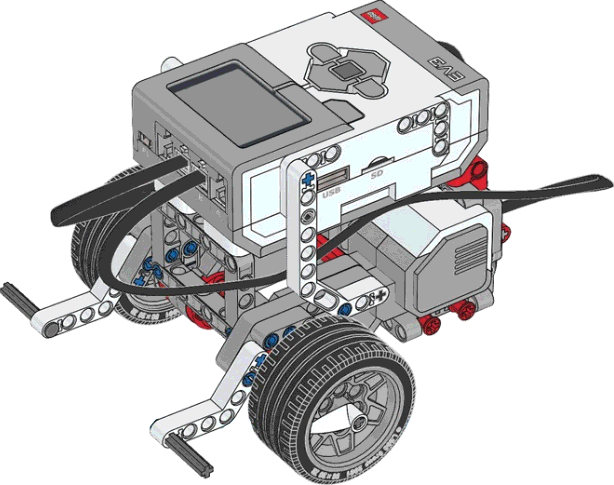
\includegraphics[width=200px]{title-page-ev3.png}					
		}
		\date{17/10/2017}
		\author{
			\bf{Team: PG-29} \\
			Benjamin Winding \\
			Kin Leong Lee \\
			Pavitterjeet Sidhu \\
			Phan Huy Nguyen \\
			Sean Hennessy \\
			Xiaoshan Chen \\
		}
		\maketitle
		
	\end{titlepage}
		 
	\tableofcontents	
	
	
	
	\section*{Revision History}	
	\label{revtable}	
	\begin{tabular}{|p{2.1cm}|p{2.5cm}|p{2cm}|p{4.1cm}|}		
		\hline 
		\textbf {Name} & \textbf{Date} & \textbf {Version} &\textbf {Summary of Changes} \\ 
		\hline 
		\hline 		
	\end{tabular}

	\newpage
	
	\section{GENERAL INFORMATION}
		\subsection{System Overview}
        This system consist two components a) The LEGO Mindstorm robot and the software to control it. The main aim of this system is to survey the specified area and safely return back to landing zone. The system is fully developed, tested and operational. GUI is also included in the system in-order to control the robot.
        The main features of this robot include
	\begin{itemize}
		\item Automatic survey of specified areas
		\item Remote control manual override and movement
		\item On-board obstacle avoidance mechanisms 
		\item No-go zone detection and avoidance
		\item Ability to return to the starting point or any point selected on mapped area.
\end{itemize}
   

        \subsection{Organization of the Manual}
        \subsubsection{User’s Manual v1.0.}
        \begin{itemize}
		\item Section 1 includes general information about the system
		\item Section 2 includes system summary
		\item Section 3 includes how to set up the system
		\item Section 4 includes how to use the system
\end{itemize}
        \subsection{Definitions, Acronyms and Abbreviations}
        \subsubsection{Definitions}
\begin{itemize}
\item Intellij IDE - Java(IDE) for developing computer software
\end{itemize}

\subsubsection{Acronyms}
\begin{itemize}
\item RMS - Robot Mapping System
\item OS - Operating System
\item JRE - Java Runtime Environment
\item IDE - Integrated development environment
\item NGZ - No Go Zone
\item SDD - Software Design Document
\item SRS - Software Requirements Specification
\item WDDM - Windows Display Driver Model
\end{itemize}

\subsubsection{Abbreviations}
\begin{itemize}
	\item min - minute
\end{itemize}
    \newpage    
	\section{SYSTEM SUMMARY}
		\subsection{System Configuration}
        The system features a GUI which can be used to instruct the robot. The user can simple click the connect button to connect the robot through the wifi but the only condition is that the  computer and the robot should be connected to the same network. User can load a new survey map to the system using the load map button on GUI. User can also set NGZ using corresponding button. 
        \subsection{Data Flows}
        User can provide input using the keyboard of the computer and using the mouse as well. The information such as robot's location on the survey map, data from the sensors of the robot will be visible on the GUI in real time.
        \subsection{User Access Levels}
        The is no security and authentication level included in the system.
        \subsection{Contingencies }
        The only factor which may degrade the performance of the system is the network speed. In the case of an emergency during the survey, a stop button is included in the GUI which will immediately stop the robot. 
     \newpage 
  \section{GETTING STARTED} 
  This section is to provide instructions from initiation to exit. The reasonable arrangement of instructions allows users to understand the flow of the system and how to control robot better.
 
  \subsection{Logging On} 
  Same wireless network environment is required for the robot and the program. Users need to ensure the robot and the computer in the same network environment.    
   
  \begin{figure}[H] 
  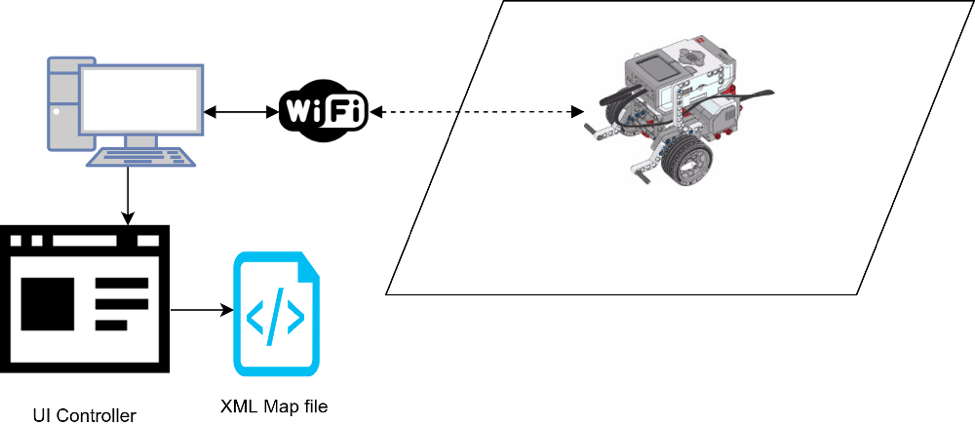
\includegraphics[width=\linewidth]{wireless.png}  % created using www.draw.io 
  \caption{Connection Overview} 
  \label{fig:Connection Overview}               
\end{figure} 
   
  \subsection{Exit System} 
  Click on Exit.
 
   
  \newpage 
  \section{USING the SYSTEM} 
  This section provides a detailed description of the robot system functions, which including the GUI functions and features that the robot has.
 
   
  \subsection{System Design} 
  This section is to describe the whole GUI design, allowing the user control the robot easily. Different parts of GUI will be shown below.
 
  \subsubsection{System Status} 
  This part is design for allowing the user know the connected status between the robot and the computer, including state of the system connection, the color sensor, and the ultrasonic sensor. When the status are connected, the icon will be changed from red to green.
   
  \begin{figure}[H] 
  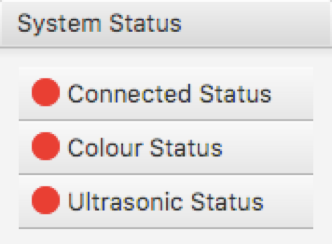
\includegraphics[width=\linewidth]{systemconnect.png}  % created using www.draw.io 
  \caption{System Connection} 
  \label{fig:System Connection}               
  \end{figure} 
   
  \subsubsection{System Mode} 
  This part is for the user to switch mode, including manual mode and automatically mode. The user can click one of modes to control the robot.
  \begin{figure}[H] 
  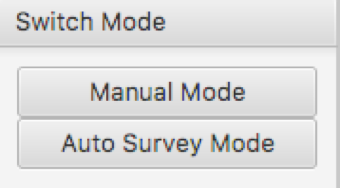
\includegraphics[width=\linewidth]{mode.png}  % created using www.draw.io 
  \caption{Mode Switch} 
  \label{fig:Mode Switch}               
  \end{figure} 
  
  \subsubsection{  Manual Controls} 
This part is for the user to control the robot manually, including up, down, turning left and turning right. The red button in the middle is for stopping the robot for the user.
  \begin{figure}[H] 
  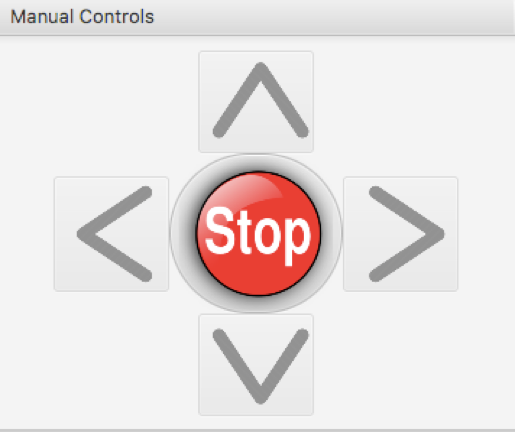
\includegraphics[width=\linewidth]{buttons.png}  % created using www.draw.io 
  \caption{Manual Buttoons} 
  \label{fig:Manual Buttoons}               
  \end{figure} 
   
   
  \subsubsection{Log Events} 
This part is for showing the system log, sensor graphs, and the current location of the robot on the map. The user can check the log and status when the robot is surveying on the map.
  \begin{figure}[H] 
  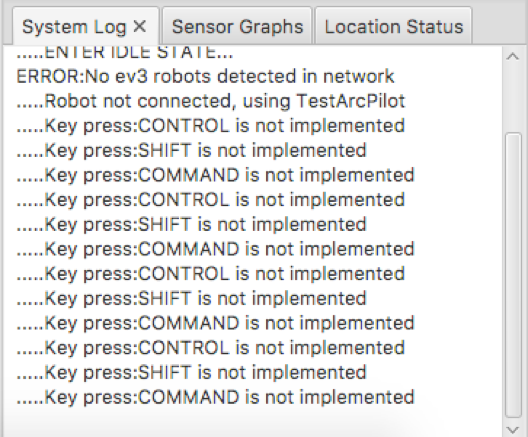
\includegraphics[width=\linewidth]{log.png}  % created using www.draw.io 
  \caption{Log Events} 
  \label{fig:Log Events}               
  \end{figure} 
   
   
  \subsubsection{  Map Options} 
This part is for showing the system log, sensor graphs, and the current location of the robot on the map. The user can check the log and status when the robot is surveying on the map.
  \begin{figure}[H] 
  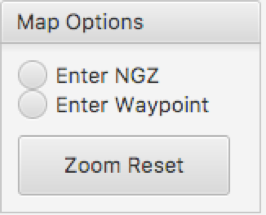
\includegraphics[width=\linewidth]{options.png}  % created using www.draw.io 
  \caption{Map Options} 
  \label{fig:Map Options}               
  \end{figure} 
   
   
  \subsubsection{  System Mode} 
This part is for showing the system log, sensor graphs, and the current location of the robot on the map. The user can check the log and status when the robot is surveying on the map.
  \begin{figure}[H] 
  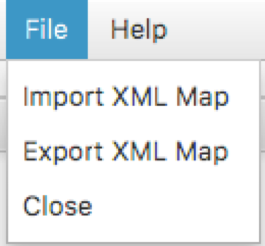
\includegraphics[width=\linewidth]{xml.png}  % created using www.draw.io 
  \caption{XML Map} 
  \label{fig:XML Map}               
  \end{figure} 
  
 
 
  \subsection{System Features} 
   
  \subsubsection{Manual Enter NGZ} 
  The user is able to designate the NGZ any time for avoiding potential dangerous areas of map detected by the remote operator.
 
  \begin{figure}[H] 
  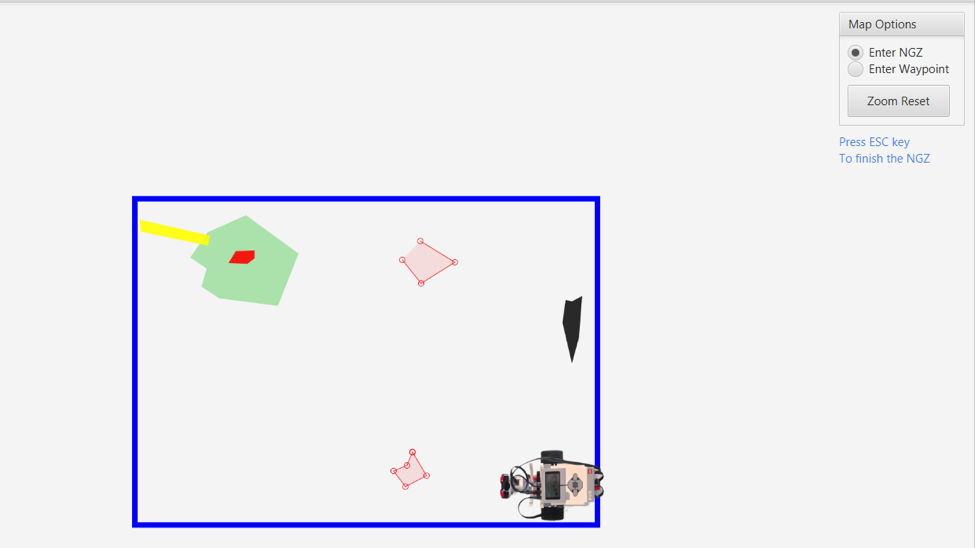
\includegraphics[width=\linewidth]{enterngz.png}  % created using www.draw.io 
  \caption{Enter NGZ} 
  \label{fig:Enter NGZ}               
  \end{figure} 
 
  \subsubsection{Avoiding the NGZ} 
The robot can avoid the NGZ when the robot is in automatically controlled.
  \begin{figure}[H] 
  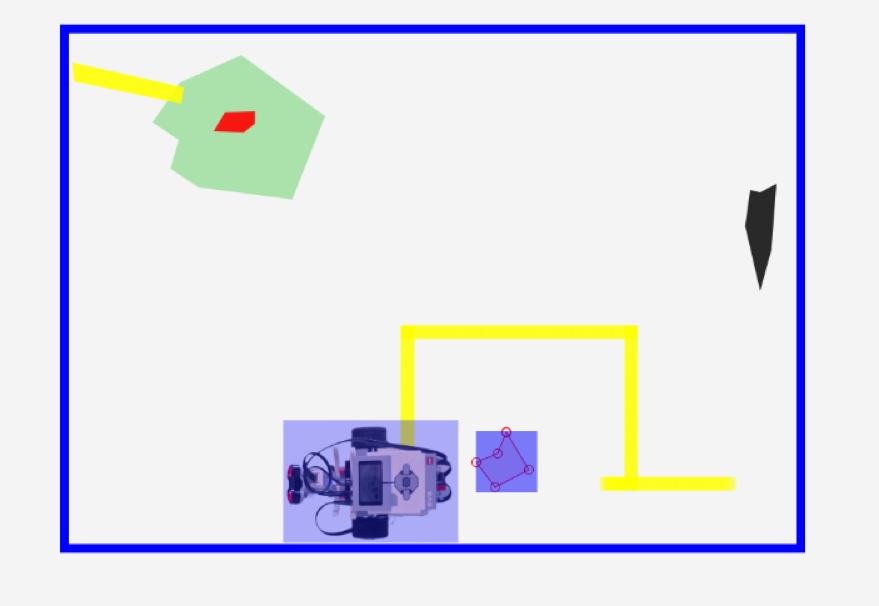
\includegraphics[width=\linewidth]{avoidngz.png}  % created using www.draw.io 
  \caption{Avoid NGZ} 
  \label{fig:Avoid NGZ}               
  \end{figure} 
   
  \subsubsection{  Move to Waypoint} 
When the user designated a waypoint, the robot can go to the waypoint directly.
  \begin{figure}[H] 
  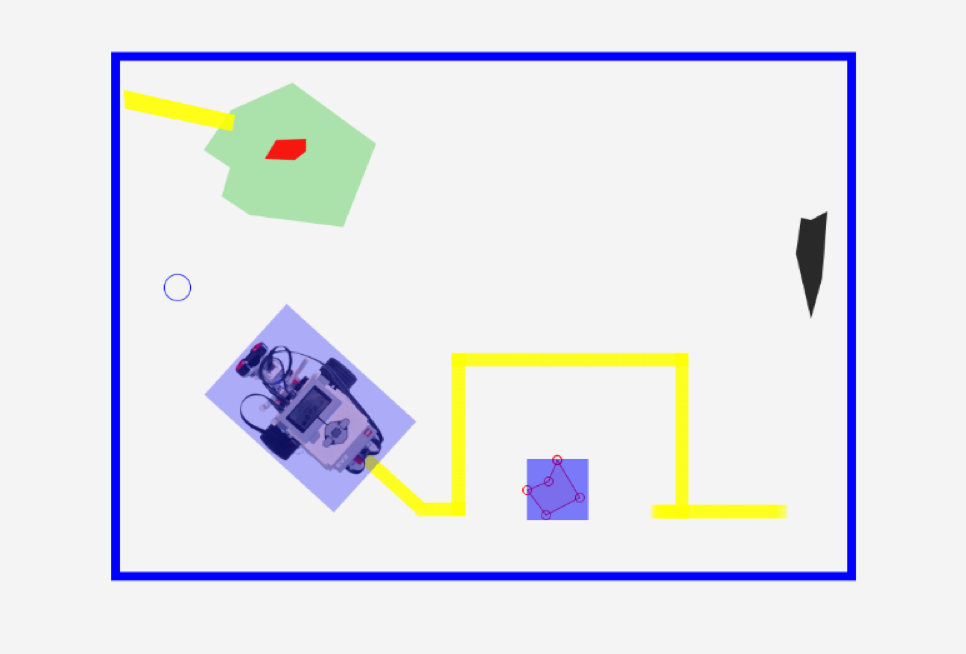
\includegraphics[width=\linewidth]{waypoint.png}  % created using www.draw.io 
  \caption{Waypoint} 
  \label{fig:Waypoint}               
  \end{figure} 
  
  
  
	\subsubsection{  Displaying the Red Color} 
The robot will change red when the robot is closing to the crater, NGZ, or the obstacle.
  \begin{figure}[H] 
  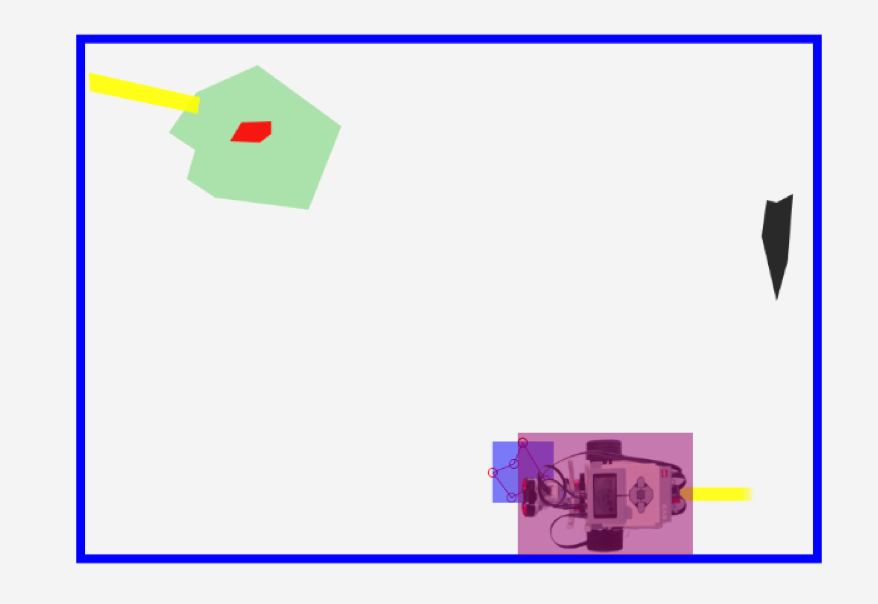
\includegraphics[width=\linewidth]{red.png}  % created using www.draw.io 
  \caption{Display Red} 
  \label{fig:Display Red}               
  \end{figure} 
   
  \subsection{Special Instructions for Error Correction} 
  As a condition of your use of the Robot, you will not use the robot for any purpose that is prohibited or unlawful by these terms, conditions, and notices. You may not do any manner that could overburden, or impair, damage of the Robot. You will not be permitted to gain unauthorised access to the Robot.  
  
 
   
  \newpage 
  \section{Appendices} 
  Instructions flow: 
  \begin{figure}[H] 
  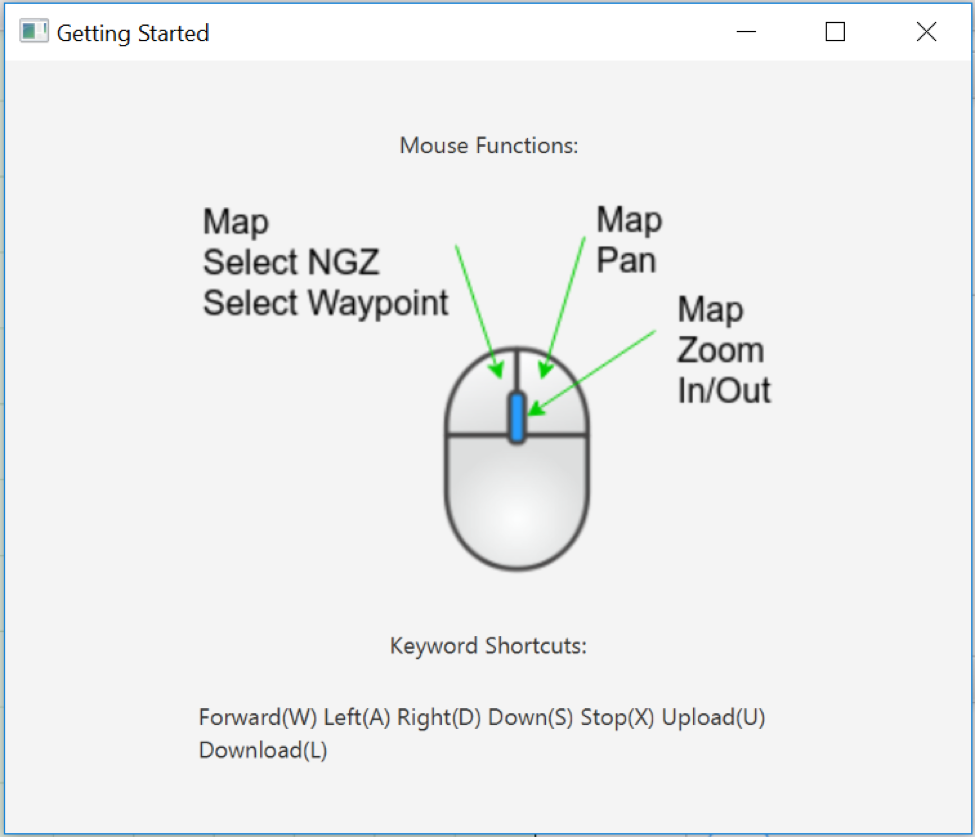
\includegraphics[width=\linewidth]{instructions.png}  % created using www.draw.io 
  \caption{Instructions} 
  \label{fig:Instructions}               
\end{figure} 
		
	
\end{document}
